\subsection{Systematic Uncertainties}
\label{sec:systsUnc}
\par Systematic uncertainities considered in this analysis are grouped into 
 experimental and theoretical categories. Regardless of the category, the procedure for evaluating 
each uncertainty's impact on the analysis results is the same:
\begin{enumerate}
\item  a parameter that corresponds to that uncertainty is shifted by $\pm 1\sigma$ from the 
nominal value; 
\item this shift may propagate to the final event yields, 
the shapes of key kinematic distributions such as \mT, or both; 
\item and finally, shape 
and yield shifts are both examined for each systematic variation in this analysis.  
\end{enumerate}

\subsubsection{Experimental Systematic Uncertainties}
\par Experimental systematic uncertainties include uncertainties on reconstruction efficiencies, 
identification efficiencies, energy scales, or momentum scales of all the physics objects 
used in the analysis. These objects are electrons, jets, and the \tauvis. These variations were propagated 
to the hard term component of \met. An additional uncertainty was also considered on the \met\ soft 
term. The uncertainty due to $b$-tagging efficiency was also considered. Table~\ref{tab:expUnc} 
shows the impact of the most dominant uncertainties on \ttbar\ and several of the expected yields. 
Uncertainties related to electrons and muons were found to be negligibly small. 

\begin{table}[!h]
\begin{center}
  \resizebox{\textwidth}{!}{
\begin{tabular}{|l|cc|cc|cc|cc|}
\hline
\multirow{2}{*}{Variation} & \multicolumn{2}{c|}{\ttbar}& \multicolumn{2}{c|}{Signal $\mcH=400~\GeV$}   & \multicolumn{2}{c|}{Signal $\mcH=1000~\GeV$} & \multicolumn{2}{c|}{Signal $\mcH=2~\TeV$}  \\
													 & up (\%) & down (\%)       & up (\%) & down (\%)       &up (\%) & down (\%)       &up (\%) & down (\%)       \\
\hline\hline
\tauvis\ reconstruction efficiency & -2.8 & 2.8 & 2.4 & 2.4 & -2.1 & 2.1 & -2.2 & 2.2 \\
\tauvis\ ID efficiency & -11.2&11.2 & -7.7& 7.7 & -7.3 & 7.3 & -8 & 8 \\
\tauvis-lepton OLR & -1.2 & 1.2 & -1.7 & 1.7 & -2.3 & 2.3 & -2.4 & 2.4 \\
\tauvis\ energy scale & -6.4 & 6.1 & -4.8 & 4.0 & -1.2 & 1.5 & 1.8 & -0.4 \\
\hline 
Jet energy scale & -10 & 11 & -4.4 & 4.8 & -1.8 & 2.6 & -1.1 & 1.9 \\
$b-$tagging efficiency & -2 & 2 & 2 & -2 & 1.7 & -1.6 & 1.5 & -1.5 \\
\met\ soft term scale/resolution & $2.1$ & $-2.1$ & -1.6 & 1.6 &  $<0.1$ & $<0.1$ &  $<0.1$ & $<0.1$ \\
Trigger efficiency & -3 & 3 & -1 & 1 & 0.2 & 0.2 &  $<0.1$ & $<0.1$ \\ 
\hline
\end{tabular}
}
\end{center}
\caption{Experimental systematic uncertainties.}
\label{tab:expUnc}
\end{table}


\par The procedures for obtaining systematic uncertainties for \tauvis, jet and b-tagging are 
discussed in Chapter~\ref{obj}.   

\par The systematic uncertainty associated with the trigger efficiency is a combination of the following 
uncertainties :
\begin{enumerate}
\item statistical uncertainties in each bin of the efficiency distribution; 
\item identification of \tauvis\ in the control region used to measure the trigger efficiency;
\item identification of the electron in the said control region; 
\item and jet reconstruction in the said control region. 
\end{enumerate}  

Statistical uncertainties in each bin of the turn-on curve are assummed to follow a Poisson 
distribution. Identification of the \tauvis\ was evaluated by varying its identification 
criteria from loose to medium, and tight. The same variation technique was applied to 
the electron object. The number of reconstructed jets requirement was varied between a minimum 
of two and three. %The effect of these variations is shown in Figure~\ref{fig:trigVars}

\par Uncertainties associated with fake factors, described in Section~\ref{sec:jetToTau}, were also 
 observed to be significantly large. 
As already mentioned, the object from which the reconstructed jet is initiated (light flavor 
quark, heavy flavor quark or gluon) affects the values of the measured fake factors. The minimum 
jet BDT score required for jets in the anti-$\tau$-id region was varied to allow different composition 
of reconstructed jets. Since the nominal selection is 0.5, the $\pm 1\sigma$ variations were taken 
as 0.4 and 0.6 respectively. These variations affect both the shape of the \mT\ distribution in 
the signal region, and the overall yield of accepted events. The effect on the latter is about 20\%. 
The effect of the former is shown in Figure~\ref{fig:bdtFF}. 
The number of \tauvis\ matched to true $\tau$ leptons in $N^{\text{anti-}\tau}_{\text{fakes}}$, when 
computing $N^{\tau}_{\text{fakes}}$ in Equation~\ref{eq:ffDef} was also generously varied by 50\%. 
This variation affects both the shape of the \mT\ distribution in the signal region and the final 
accepted event yield. The latter is shifted by about 6\%. The last significant source  of uncertainty in 
the fake factor method is due to statistical uncertainties in the measurement control samples. This only 
affects the event yield by about 3\%. No \mT\ shape shifts were observed.   

\begin{figure}[!h]
\centering
   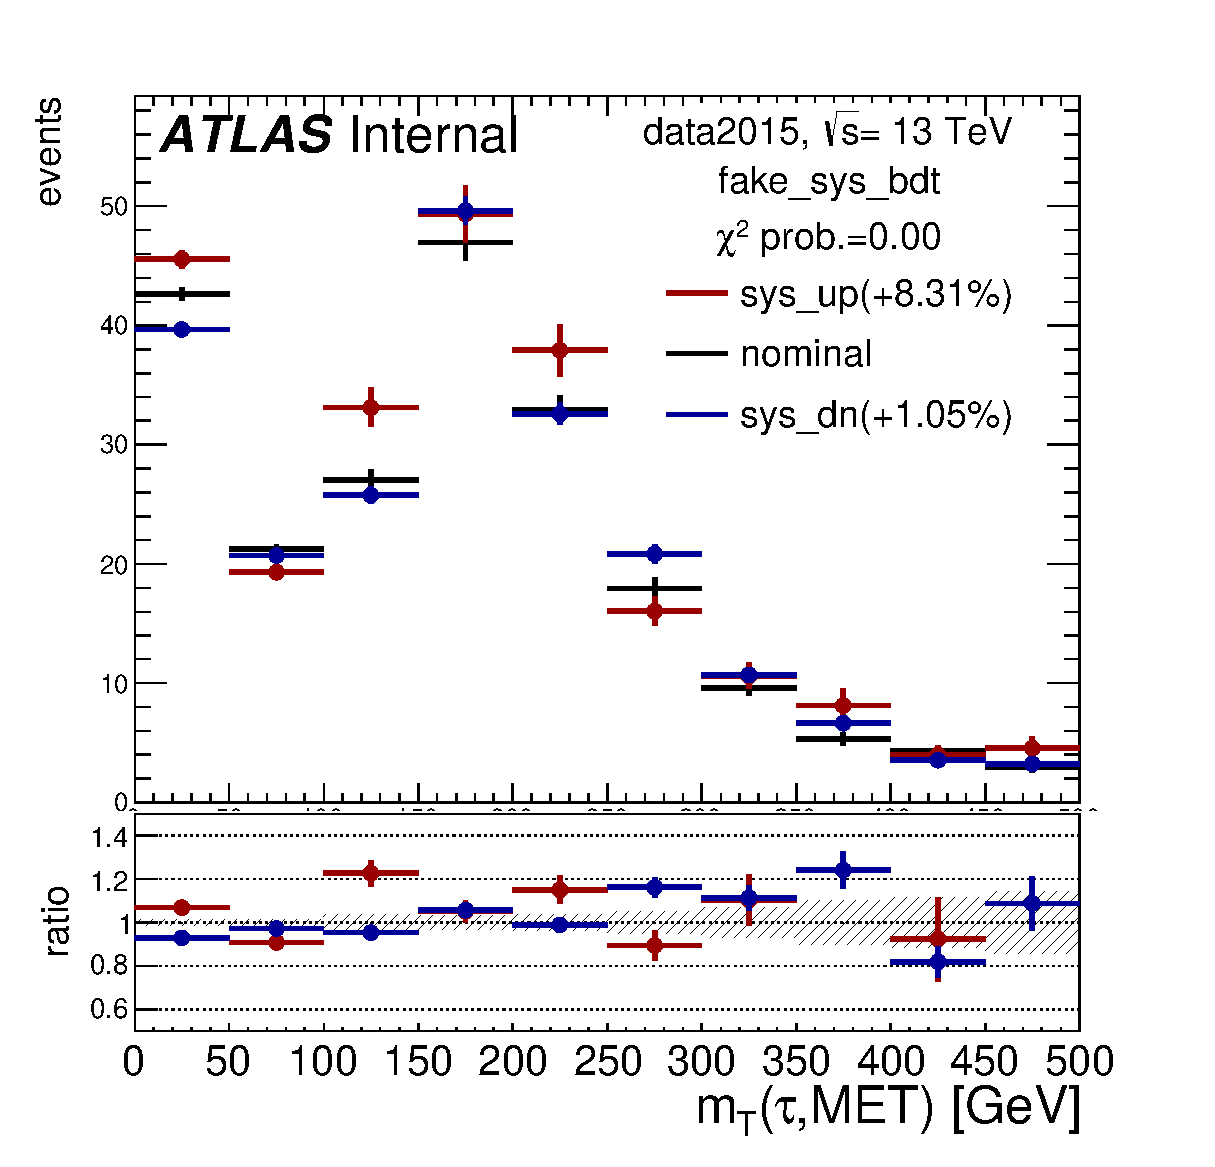
\includegraphics[width=0.8\textwidth]{figures/Syst_fake_sys_bdt.eps}
\caption{Plots showing \mT\ distributions with variation in jet BDT score selection criteria}
\label{fig:bdtFF}
\end{figure}

\subsubsection{Theoretical Systematic Uncertainties}
\par Theoretical uncertainties include uncertainties due to the choice of the QCD renormalization
 and factorization scales, choice of parton distribution functions, and tunes applied to the parton 
shower and underlying event models. These uncertainties were computed for signal samples and the most 
dominant backgrounds, which are \ttbar\ and \Wjets.    

\par For signal samples, the QCD renormalization scale $\mu_R$ and factorization scale $\mu_F$ were 
varied by a factor of 0.5 and 2.0 to evaluate their impact on the expected signal yields. 
This impact was shown to be less than 5\%. Table~\ref{tab:scalesSig} shows the percentage impact 
on the individual variations on several \mcH.  The largest variation was symmetrized and 
taken as the QCD scale uncertainty for that mass point.  

\begin{table}[!h]
\begin{center}
  \resizebox{\textwidth}{!}{
\begin{tabular}{|l|cccccccc|}
\hline
Mass  & \multicolumn{8}{c|}{$\mu_R\times\mu_F$ (\% diff)}  \\
(GeV) & $0.5\times0.5$ &  $0.5\times1.0$ & $0.5\times2.0$ & $1.0\times0.5$ & $1.0\times2.0$ & $2.0\times0.5$ & $2.0\times1.0$ & $2.0\times2.0$ \\
\hline\hline
200 & -8 & 1.7 & 7 & -7 & 4 & -8 & -2 & 2 \\
500 & -5 & -1 & 2 & -3 & 2 & -2 & 1 & 2 \\
800 & -4 & -1 & 1 & -2 & 1 & -1 & 1 & 2 \\
1000 & -4 & -1.3 & 0.6 & -2 & 1.5 & 0.7 & 1 & 2 \\
\hline
\end{tabular}
}
\end{center}
\caption{Theoretical systematic uncertainties on the signal acceptance (in \%) due to the QCD scale. 
The factorization scales are varied by a factor of 2 for up and down variations.}
\label{tab:scalesSig}
\end{table}

\par Dependence on the parton distribution function (PDF) set choice is evaluated by LHAPDF~\cite{Buckley:2014ana}. 
For a sample generated with PDF set $A$, LHAPDF is able to compute weights for each event, such that
the dataset would equivalent to a dataset generated with PDF set $B$. By taking NNPDF23\_nlo\_as\_0118\_qed 
 as the nominal PDF set, 3 variations were then examined : NNPDF30\_nlo\_as\_0118\_nf\_4, 
CT14nlo\_NF4, and MSTW2008nlo68cl\_nf4. The largest variation was symmetrized and taken as the error 
on the PDF choice. This variation was found to have less than 1\% impact on the results 
for all signal samples.  

\par Uncertainties due to parton shower and underlying event tunes were considered for 
$\mcH=200, 500,$ and 800~\GeV. The A14 tune with the NNPDF set comes with a set of 
systematic variations that were empirically found to cover the total uncertainty in the data used to 
tune parton shower and underlying event models. A pair of these variations, {\it Var1}, covers 
underlying event effects. Another pair, {\it Var2}, covers jet structure effects. 3 other pairs, {\it Var3a, Var3b} and 
{\it Var3c}, cover aspects of extra jet production. The up and down variations were symmetrized and summed in quadrature to obtain 
their full impact. Table~\ref{tab:systsPS} summarizes the percentage impact of each symmetrized variation. 

\begin{table}[!h]
\begin{center}
\begin{tabular}{|l|ccccc|}
\hline
Mass (GeV)  & Var1 (\%) & Var2 (\%)& Var3a (\%) & Var3b (\%) & Var3c (\%)  \\
\hline\hline
200 & 2 & 7 & 8 & 10 & 10 \\
500 & 4 & 4 & 5 & 4  & 6  \\
800 & 4 & 4 & 5 & 8 & 1 \\
\hline
\end{tabular}
\end{center}
\caption{Theoretical systematic uncertainty on the signal acceptance due to choice of parton shower and 
underlying event tune.}
\label{tab:systsPS}
\end{table}

\par QCD scale, choice of parton shower and underlying event tunes, and choice for matrix element generator 
were evaluated for \ttbar. The impact on the predictions was evaluated by generating Monte Carlo simulation samples    
with the respective variations and imposing signal region selection criteria on them. 
 \POWHEG+\PYTHIA\ version 8 
samples were used as the nominal samples. Separate samples with more final state radiation (FSR) and 
less FSR were also generated. \MGMCatNLO+\HERWIGPP\ and \POWHEG+\HERWIGPP\ samples 
were generated to evaluate the impact of using different matrix element generators.    
The impact of using different parton showering and underlying event tunes was computed 
by comparing \POWHEG+\PYTHIA version 8 and \POWHEG+\HERWIGPP samples. QCD scale and PDF choice 
uncertainties were shown to be less than 5\%. Shift on the event yield due to FSR was shown to be 
approximately 7\%, for the choice of matrix element generator it was 15\%, and for the choice of 
parton shower and underlying event tunes it was 16\%. Effects of these variations on the shape 
of the $\mT(\tau,\nu)$ distribution were also examined, after normalizing the samples to the same 
NNLO+NNLL cross section.% Figures~\ref{fig:shapeTTBarA}, \ref{fig:shapeTTBarB}, \ref{fig:shapeTTBarC}
% shows these shape differences.    

\par Various selection criteria in the \Wjets\ control region were varied to evaluate the 
systematic uncertainties on the \Wjets\ background. All these variations were shown to be 
less than 3\%. Since contributions from other background process in the signal region are 
very small, their systematic variations were taken as negligible. 

\subsection{Statistical Methods}
\par The \mT\ distributions for signal samples with $200<\mcH<2000~\GeV$, and background processes
 in the signal region are used to test for the presence of charged Higgs bosons with \mcH\ in the 200$\to$2000~\GeV mass range 
in data. This procedure involves tests on two hypotheses : that the data is fully 
described by the known Standard Model processes, called the {\it background-only} ($b$) hypothesis; and that some 
signal is required to explain the observed data, called the {\it signal+background} ($s+b$) hypothesis. 
Since the signal true cross section $\sigma_{H^+}^{Obs}$ is not known a-priori, a parameter of interest (POI)  

\begin{equation}
\mu = \frac{\sigma_{H^+}^{Obs}}{\sigma^{Exp}_{H^+}}
\end{equation}

is defined to parametrize the $s+b$ hypothesis into $\mu.s+b$. Here, $\sigma^{Exp}_{H^+}$ is the 
expected cross section from phenomenological models introduced in Chapters~\ref{theory}. A test can be made independent of 
$\sigma^{Exp}_{H^+}$ by setting it equal to 1; this would make the POI $\mu$ equal to the true 
cross section $\sigma_{H^+}^{Obs}$. In any case $\mu\geq 0$, where $\mu=0$ reduces the $s+b$ hypothesis to the 
background-only hypothesis. 

\par Since the number of events in the signal region is usually small, the \mT\ distributions used  for these 
tests are optimally binned to minimize statistical uncertainties. For an \mT\ distribution with $N$ bins, 
the expected number of events in each bin can be parametrized as   

\begin{equation}
E_i = \mu.s_i + b_i
\end{equation} 

where $i$ runs from 0 to $N$. Variables $s_i$ and $b_i$ are the expected signal 
and background events in the $i-$th bin respectively. These events follow a Poisson probability distribution 
with means $s_i$ and $b_i$ respectively. The statistical methods described here are based on the {\it binned likelihood 
function, L}, which is a product of Poisson probability terms over all the $N$ bins    

\begin{equation}
L(\mu) = \prod_{i=0}^N \frac{(E_i)^{n_i}}{n_i!}\exp (-E_i)
\end{equation}

\par $s_i$ and $b_i$ are affected by the systematic uncertainties discussed in Section~\ref{sec:systsUnc}. 
More specifically, the $s_i$ and $b_i$ probability distributions become wider when the systematic uncertainties 
are accounted for. A set of $P$ systematic uncertainties can be included in the statistical 
method as {\it nuisance parameters}, $\theta = (\theta_1,...,\theta_P)$, transforming $s_i$ and $b_i$ 
as $s_i\to s_i(\theta)$ and $b_i\to b_i(\theta)$ respectively.   
Likewise, the binned likelihood function is transformed as  

\begin{equation}
L(\mu) \to L(\mu,\theta) = \prod_{i=0}^N \frac{(\mu.s_i(\theta) + b_i(\theta))^{n_i}}{n_i!}\exp(\mu.s_i(\theta) + b_i(\theta)).\prod_{k=1}^P\rho(\theta_k).
\end{equation}

\par From the binned likelihood function a test statistic called the {\it profile likelihood ratio}

\begin{equation}
q_\mu = -2\ln\left (\frac{L(\mu,\hat{\hat{\theta}}}{L(\hat{\mu},\hat{\theta})} \right )
\label{eq:testStat}
\end{equation}

is created, where $\hat{\mu}$ and $\hat{\theta}$ are parameters that maximize the likelihood functions. 
The $\hat{\hat{\theta}}$ parameters are the nuisance parameters that maximize the likelihood function for a given $\mu$ value. 
 
\par The compatibility between data and a given hypothesis is quantified by computing a $p$-value. 
This is the probability of observing results as incompatible with data or worse, given that said hypothesis. 
For the $s+b$ hypothesis, the $p$-value is 
 
\begin{equation}
p_{s+b} = \int_{q_{\text{obs}}}^{\infty} f(q|s+b)dq
\label{eq:sPb}
\end{equation}

where $f(q|s+b)$ is the probability distribution function of the test statistic $q$ given the $s+b$ 
hypothesis. For the $b$ hypothesis the $p$-value is 

\begin{equation}
p_{b} = \int_{q_{\text{obs}}}^\infty f(q|b)dq
\label{eq:b}
\end{equation}

where $f(q|b)$ is the probability distribution function of the test statistic $q$ given the $b$ 
hypothesis. Figure~\ref{fig:pVal} illustrates how these $p_{b}$ is computed from a distribution 
of $f(q|b)$ and an observed $q_{\text{obs}}$ in data. 

\par These $p$-values are converted to a {\it significance}, defined as the number 
of standard deviations $Z$ at which a normally distributed variable with 0 mean would give a 
one-sided tail area equal to the $p-$value. %Figure~\ref{fig:zscore} illustrates the relationship 
%between $Z$ and $p$.   

\begin{figure}[h]
\centering
   \includegraphics[width=0.8\textwidth]{figures/pVal_sPb.pdf}
\caption{$p_{b}$ illustration from a distribution 
of $f(q|b)$ and an observed $q_{\text{obs}}$ in data}
\label{fig:pVal}
\end{figure}

\par From Equations~\ref{eq:sPb} and \ref{eq:b} a confidence level (CL) of the $s+b$ hypothesis is 
defined as 
 
\begin{equation}
CL_s(\mu) = \frac{CL_{s+b}}{CL_b} = \frac{p_{s+b}}{1-p_b}
\label{eq:cls}
\end{equation}

A 95\% CL upper limit on $\mu$ is set by finding the $\mu$ at which $CL_s = 0.05$, using the 
asymptotic approximation. 
